
\documentclass[12pt]{article}
\usepackage[utf8]{inputenc}
\usepackage{upquote}
\usepackage[margin=20mm]{geometry} 
\usepackage{amsmath,amsthm,amssymb}
\usepackage{graphicx}
\usepackage{listings}
\newenvironment{statement}[2][Statement]{\begin{trivlist}
\item[\hskip \labelsep {\bfseries #1}\hskip \labelsep {\bfseries #2.}]}{\end{trivlist}}
\usepackage{xcolor}

\usepackage{subfigure}


% Listings package for code rendering (No external dependencies)
\usepackage{listings}  
\usepackage{xcolor}   % Color support
\usepackage{tcolorbox} % Box for better appearance

% Define custom colors for code highlighting
\definecolor{codegreen}{rgb}{0,0.6,0}
\definecolor{codegray}{rgb}{0.5,0.5,0.5}
\definecolor{codepurple}{rgb}{0.58,0,0.82}
\definecolor{backcolour}{rgb}{0.95,0.95,0.92}


\lstset{frame=tb,
    language=Python,
    backgroundcolor=\color{backcolour},   
    commentstyle=\color{codegreen},
    keywordstyle=\color{magenta},
    numberstyle=\tiny\color{codegray},
    stringstyle=\color{codepurple},
    basicstyle=\ttfamily\footnotesize,
    breakatwhitespace=false,         
    breaklines=true,                 
    keepspaces=true,                 
    numbers=left,       
    numbersep=5pt,                  
    showspaces=false,                
    showstringspaces=false,
    showtabs=false,                  
    tabsize=2,
}





\title{Assignment 5}


\author{Author \\
 Wanjing Hu / fng685@alumni.ku.dk  \\
 Shuangcheng Jia / bkg713@alumni.ku.dk/   \\
 Zhigao Yan / sxd343@alumni.ku.dk  \\
} 

\begin{document}
\maketitle

\section{Inspecting Spectrograms}
%Shuangcheng
\section{Inverse filtering}
%zhigao

\section{Fixed scale feature detectors}

%Wanjing
\subsection{}

\textbf{sigma}: This is the Standard deviation of the Gaussian filter, controlling Gaussian smoothing. Higher sigma (e.g., 3) reduces noise but blurs edges, leading to thicker and fewer edges.

\textbf{low\_threshold/high\_threshold}: These two parameters determine edge connectivity. Lower thresholds (e.g., 0.05/0.2) detect more edges, including noise, while higher thresholds retain only strong edges.

\begin{lstlisting}
image = skimage.io.imread('../TestImages/Week 1/hand.tiff', as_gray=True)
edges_default = skimage.feature.canny(image)
edges_sigma3 = skimage.feature.canny(image, sigma=3)
edges_low_high = skimage.feature.canny(image, low_threshold=0.05, high_threshold=0.2)
\end{lstlisting}

\begin{figure}[h]
    \centering
    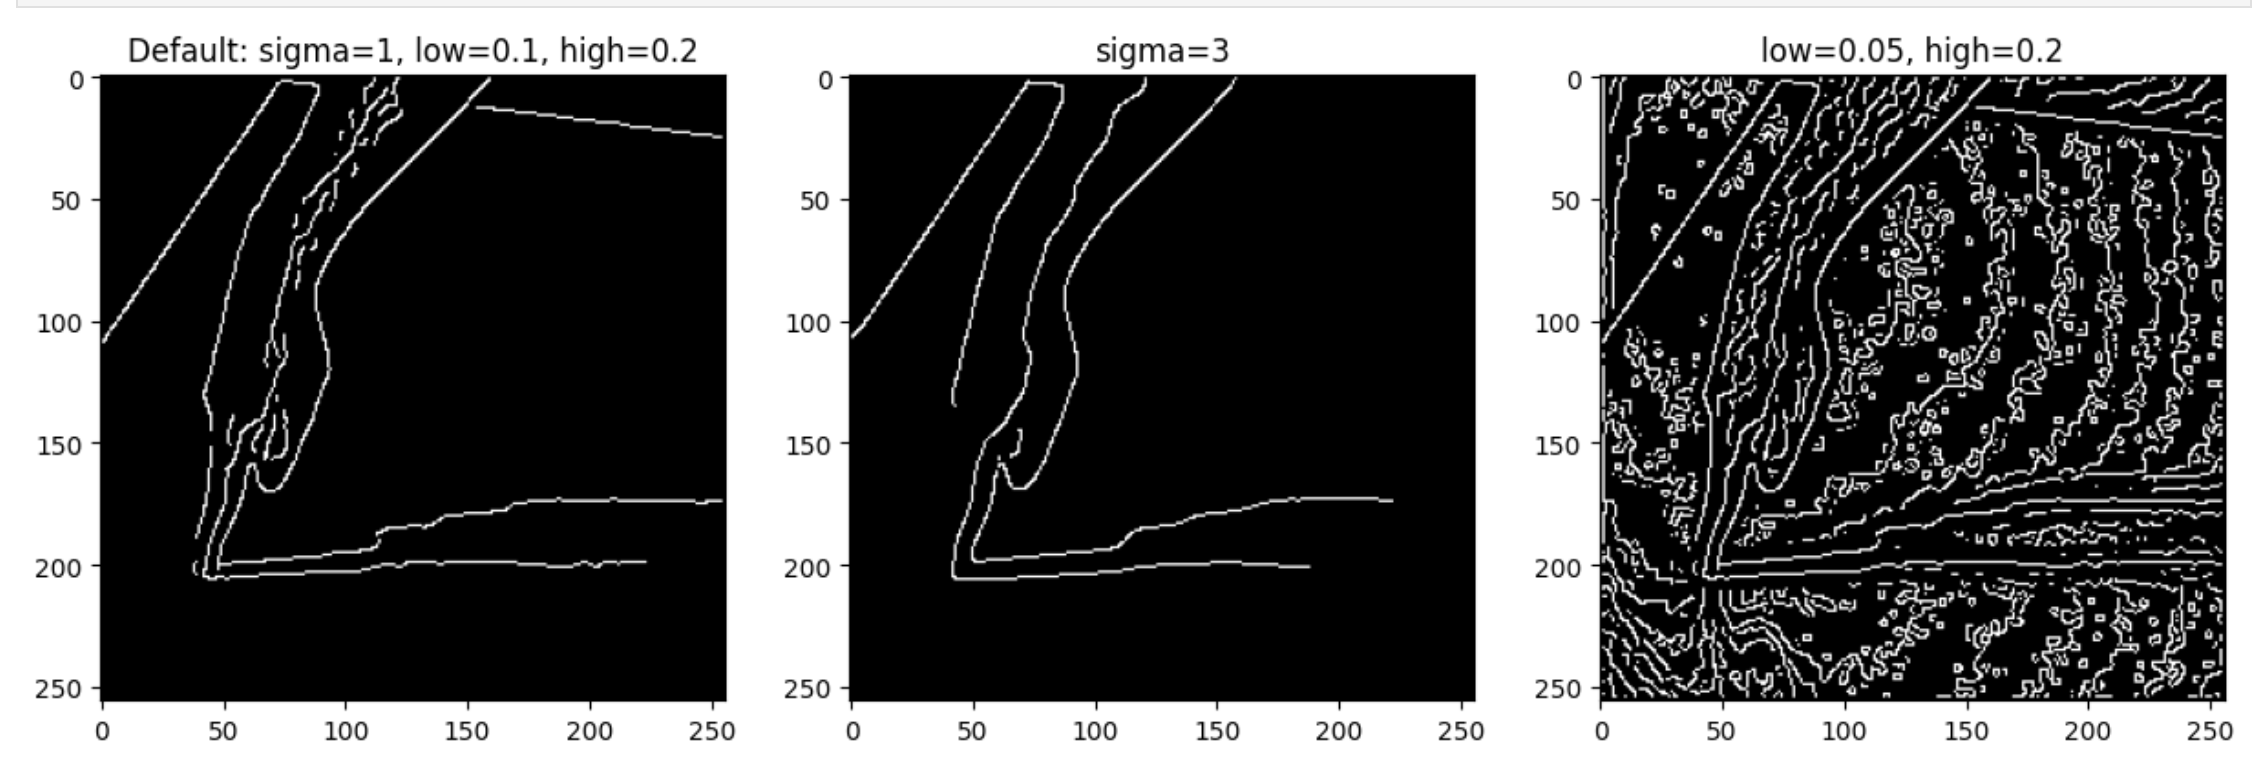
\includegraphics[width=0.6\textwidth]{pics/a5-3.1} 
    \caption{xx.}
\end{figure}

\subsection{}

\textbf{sigma}: Larger sigma (e.g., 3) smooths gradients, detecting corners at a coarser scale.

\textbf{k}: Higher k (e.g., 0.2) reduces false corners but may miss weaker ones.

\textbf{Method eps}: Uses Noble’s corner measure. The lower the eps is, the more sensitive the corner decection is.

\begin{lstlisting}
image_house = skimage.io.imread('../TestImages/Week 1/modelhouses.png', as_gray=True)

harris1 = 
	skimage.feature.corner_harris(image_house, sigma=1, k=0.05, method='k')
harris2 = 
	skimage.feature.corner_harris(image_house, sigma=3, k=0.05, method='k')
harris3 = 
	skimage.feature.corner_harris(image_house, sigma=1, k=0.2, method='k')
harris4 = 
	skimage.feature.corner_harris(image_house, sigma=1, method='eps', eps=0.01)

fig, axes = plt.subplots(2, 2, figsize=(10, 10))
axes[0,0].imshow(harris1, cmap='viridis')
axes[0,0].set_title('sigma=1, k=0.05')
axes[0,1].imshow(harris2, cmap='viridis')
axes[0,1].set_title('sigma=3, k=0.05')
axes[1,0].imshow(harris3, cmap='viridis')
axes[1,0].set_title('sigma=1, k=0.2')
axes[1,1].imshow(harris4, cmap='viridis')
axes[1,1].set_title('sigma=1, eps=0.01')
plt.show()
\end{lstlisting}

\begin{figure}[h]
    \centering
    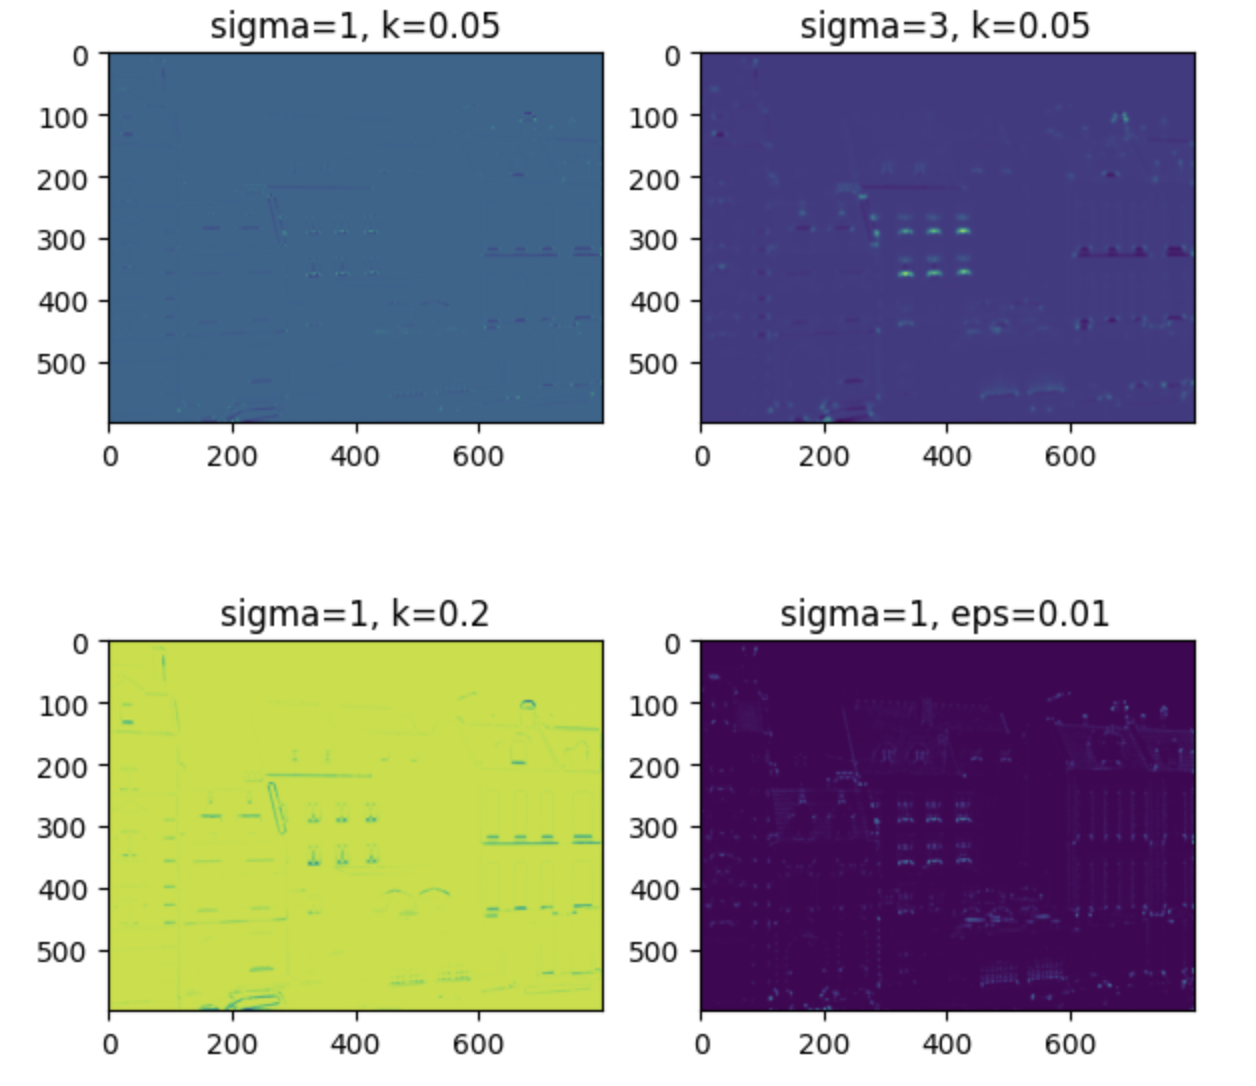
\includegraphics[width=0.6\textwidth]{pics/a5-3.2} 
    \caption{xx.}
\end{figure}

\subsection{}

The figure shows the 250 strongest Harris corners (red crosses) detected on modelhouses.png using parameters sigma=1, k=0.05, and min\_distance=1. Corners are localized at building edges and intersections.

\begin{lstlisting}
def find_harris_corners(image, sigma=1, k=0.05, method='k', min_distance=1, num_peaks=250):
    from skimage.feature import corner_harris, corner_peaks
    response = corner_harris(image, sigma=sigma, k=k, method=method)
    coords = corner_peaks(response, min_distance=min_distance, num_peaks=num_peaks)
    return coords

coords = find_harris_corners(image_house, sigma=1, k=0.05)
\end{lstlisting}

\begin{figure}[h]
    \centering
    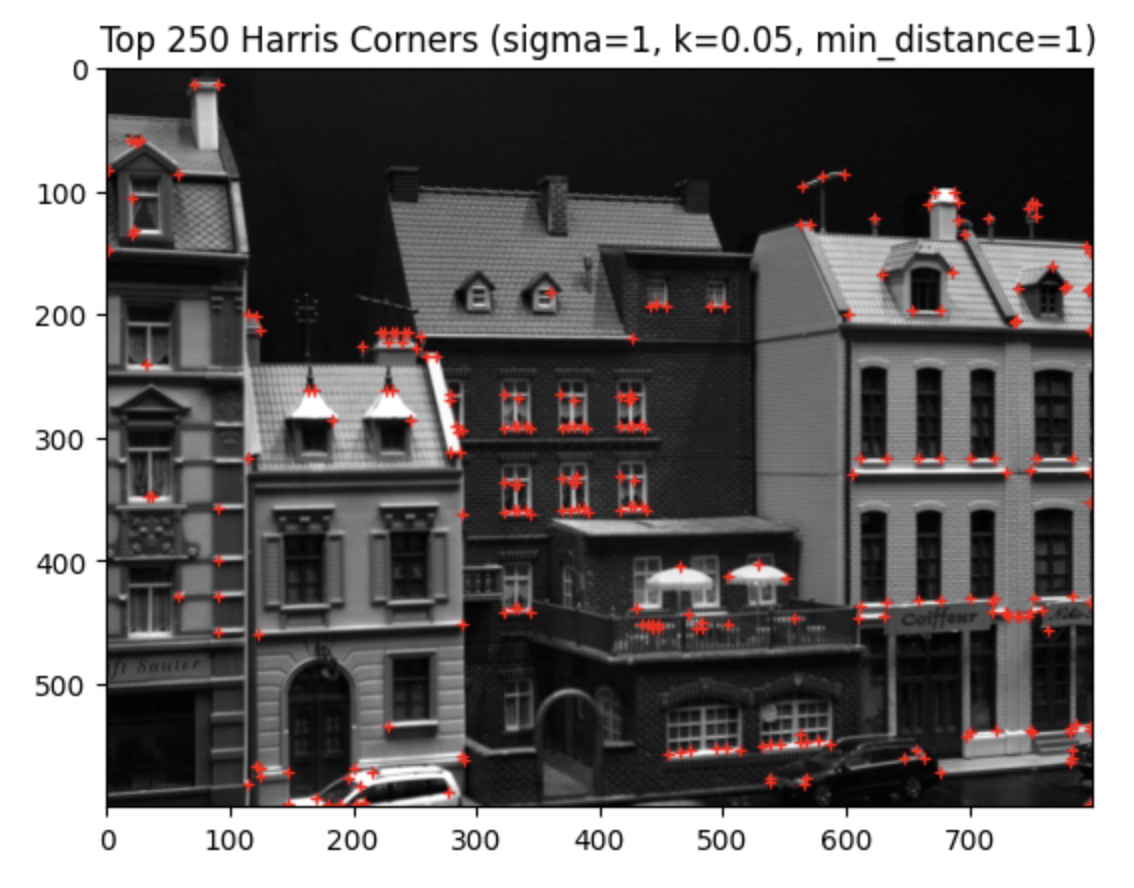
\includegraphics[width=0.6\textwidth]{pics/a5-3.3} 
    \caption{xx.}
\end{figure}

\section{Scale-space blob detector}
%Shuangcheng1

\end{document}
